\documentclass[12pt]{article}
\usepackage{graphicx, caption} % Required for inserting images
\usepackage{babel}
\usepackage{polski}
\usepackage[a4paper, right=3cm]{geometry}
\usepackage[T1]{fontenc}
\usepackage{amsmath,amsthm,amssymb}
\usepackage[utf8]{inputenc}
\usepackage{amsmath}
\usepackage{array}
\usepackage{multicol}
\usepackage{multirow}
\usepackage{float}

\title{Sprawozdanie wyznacznie współczynnika lepkości}
\author{Jan Rolka, Aleksander Pyrdek, Aleksander Mystkowski}
\date{November 2024}

\begin{document}
\renewcommand{\arraystretch}{4}%
\begin{table}[]
\scriptsize
\resizebox{\textwidth}{!}{
\begin{tabular}{|l|l|l|l|l|l|}
    \hline
    Wydział {\small \textbf{EAIIB}}                 & \multicolumn{2}{l|} {Imię i nazwisko}                                    & \multicolumn{1}{l|}{Rok {\large \textbf{II}} }         & Grupa {\large \textbf{6}}         & Zespół {\large \textbf{4}}       \\ 
    
    \hline
    {\small P. Fiz. WFiIS AGH} & \multicolumn{4}{l|}{Temat:}                                                                                                   & Nr ćwiczenia {\large \textbf{13}}  \\ 
    
    \hline
    Data wyk.:{\footnotesize \textbf{14.11.2024}}               & \multicolumn{1}{l|}{Data oddania} & \multicolumn{1}{l|}{Zwrot do popr.} & \multicolumn{1}{l|}{Data oddania} & Data zaliczenia & OCENA        \\ 
    
    \hline
\end{tabular}
}
\end{table}
\renewcommand{\arraystretch}{}%
\begin{center}
Jan Rolka, Aleksander Pyrdek, Aleksander Mystkowski
\end{center}
\section{Cel ćwiczenia}
Wyznaczenie współczynnika lepkości gliceryny metodą Stokesa, zapoznanie się z
własnościami cieczy lepkiej.
\section{Wstęp teoretyczny}

\vspace{0.5cm}

Przy przepływie wszystkich cieczy rzeczywistych ujawniają się większe lub mniejsze siły tarcia. W przeciwieństwie do ruchu ciał stałych, w którym tarcie występuje tylko na powierzchni, w cieczach i w gazach ujawnia się ono w całej objętości. Jest więc zwane tarciem wewnętrznym lub lepkością.

\vspace{0.5cm}

Współczynnik lepkości \(\eta\) jest miarą oporu, jaki ciecz stawia przepływowi. Opisuje on zależność między siłą ścinającą \(\tau\) a szybkością ścinania \(\dot{\gamma}\), zgodnie ze wzorem:
\[
\eta = \frac{\tau}{\dot{\gamma}}
\]
gdzie:
\begin{itemize}
    \item \(\tau\) — naprężenie styczne w cieczy [Pa],
    \item \(\dot{\gamma}\) — szybkość ścinania [s\(^{-1}\)].
\end{itemize}

\vspace{0.5cm}

Badanie lepkości cieczy polega na obserwacji ruchu kuli spadającej w płynie, zgodnie z prawem Stokesa. Siła oporu działająca na kulę jest proporcjonalna do współczynnika lepkości, jej średnicy oraz prędkości. Zależność ta wyraża się wzorem:
\[
F = 6 \pi \eta r v,
\]
gdzie:
\begin{itemize}
    \item \(F\) — siła oporu [N],
    \item \(r\) — promień kuli [m],
    \item \(v\) — prędkość kuli [m/s].
\end{itemize}

\vspace{0.5cm}
Wzór ten jest prawdziwy dla kulki poruszającej się w nieograniczonej objętości cieczy. Z przyczyn oczywistych nie dysponujemy basenem badanej cieczy i jej opadanie będziemy badać w cylindrze. W takiej sytuacji siła oporu jest dany wzorem.
\[F=6\pi\eta rv(1+2.4\frac{r}{R})\]
gdzie:
\begin{itemize}
    \item R-promień cylindra
\end{itemize}
Zgodnie z drugą zasadą dynamiki Newtona przyspieszenie kulki dane jest wzorem.
\[ma=F_c-F_w-F_o\]
gdzie
\begin{itemize}
    \item $F_c$-siła ciężkości
    \item $F_w$-siła wyporu
    \item $F_o$-siła oporu
\end{itemize}
alternatywnie
\[m\frac{dv}{dt}=F_c-F_w-Kv\]
gdzie
\begin{itemize}
    \item K=$6\pi\eta rv(1+2.4\frac{r}{R})$
\end{itemize}
Jest to równanie różniczkowe. Jego rozwiązanie jest postaci.
\[v(t)=v_gr+(v_0-v_gr)e^{-\frac{t}{\tau}}\]
Ruch kulki po czasie rzędu $t=3\tau$ jest w przybliżeniu ruchem jednostajnym. Oczywiście w takim ruchu przyspieszenie a=0.
\[F_c-F_w-F_o=0\]
\[mg-\rho Vg-6\pi\eta rv_{gr}(1+2.4\frac{r}{R})=0\]
\[mg-\rho\pi\frac{4}{3}r^3g-6\pi\eta rv_{gr}(1+2.4\frac{r}{R})=0\]
\[\eta=\frac{g(m-\rho\frac{4}{3}\pi r^3)}{6\pi rv_{gr}(1+2.4\frac{r}{R})}\]
Prędkość graniczna można wyznaczyć mając drogę jaką pokonuje kulka i czas.\\
Z kolei do wyliczenia objętości wystarczy średnica kulki, która jest o wiele łatwiejsza do wyznaczenia.
\[V=\frac{4}{3}\pi r^3=\frac{1}{6}\pi d\]
Z tego samego powodu warto zamienić r na $\frac{d}{2}$ oraz R na $\frac{D}{2}$
\[\eta=\frac{gt(m-\rho\frac{1}{6}\pi r^3)}{3\pi l(1+2.4\frac{r}{R})}\]

Pomiar współczynnika lepkości pozwala na charakteryzację właściwości fizycznych cieczy, takich jak jej płynność czy zdolność do tłumienia ruchu.


\section{Aparatura}

\begin{enumerate}
    \item Przyrząd do badania spadania kulki w cieczy (rys. w1)
    \item Zestaw kulek
    \item Śruba mikrometryczna
    \item Suwmiarka
    \item Waga cyfrowa
\end{enumerate}

\begin{figure}[h]
\centering
\captionsetup{width=.7\linewidth}
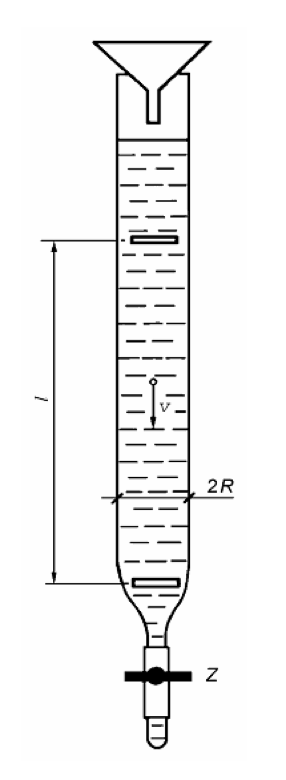
\includegraphics[scale=0.4]{rysunek1.png}
\caption{Rys. w1. Przyrząd do pomiaru współczynnika lepkości metodą Stokesa. (Z – zacisk służący do odzysku kulek)[1]}
\label{fig:example}
\end{figure}

\section{Wykonanie ćwiczenia}

\begin{enumerate}
    \item Wybrane do pomiaru kulki dokładnie wytarto z resztek gliceryny, a następnie rozłożono na arkuszu bibuły, jednocześnie nadano każdej z nich numer. Po wykonaniu jakiegokolwiek pomiaru, użyta kulka powinna zawsze zostać wytarta i odłożona na miejsce.
    
    \item Zmierzono średnice wszystkich wybranych kulek za pomocą śruby mikrometrycznej. Wyniki zapisano w Tabeli 1.
    
    \item Zważono wszystkie kulki przy użyciu dostępnej wagi. Wyniki zapisano w Tabeli 1.
    
    \item Ustawiono na rurze dwa znaczniki w odległości około 80 cm tak, aby górny znacznik znajdował się co najmniej 20 cm poniżej poziomu cieczy w rurze. Zanotowano odległość znaczników w Tabeli 1.
    
    \item Odczytano wartość średnicy używanego cylindra. Dane wpisano do Tabeli 1.
    
    \item Każdą z kulek wrzucono do rury, a następnie zmierzono za pomocą stopera czas, w którym będzie ona opadała pomiędzy znacznikami. Wynik zapisano w Tabeli 1. Zwrócono uwagę aby kulki opadały środkiem cylindra, a nie blisko ścianek oraz aby nie było do nich doczepionych pęcherzyków powietrza. Każdy pomiar, który nie spełnia powyższych wymogów powtórzono.
    
    \item Wyciągnięto kulkę z cylindra poprzez kran umieszczony na jego dolnym końcu. Aby nie dopuścić do wylewania się gliceryny z cylindra posłużono się zaciskaczem umieszczonym na wężyku. Gliceryna powinna ściekać do podstawionego pod wężykiem naczynia. Jeśli zachodzi potrzeba uzupełnienia gliceryny w cylindrze, należy przelać ją ostrożnie z naczynia lejąc po ściankach cylindra tak, aby wytworzyć jak najmniej pęcherzyków powietrza.
    
    \item Po skończonych pomiarach zanotowano temperaturę otoczenia, w której wykonywane było doświadczenie.[1]
\end{enumerate}



\section{Wyniki pomiarów:}
Droga spadania kulki = 800[mm]\\
Średnica cylindra = 34 [mm]\\
Temperatura = 22.5[C]

\vspace{0.5cm}

\textbf{Tabela 1}
\begin{table}[h]
\begin{tabular}{|c|c|c|c|c|c|}
\hline
\begin{tabular}[c]{@{}c@{}}Nr\\ pomiaru\end{tabular} & \begin{tabular}[c]{@{}c@{}}Nr\\ kulki\end{tabular} & \begin{tabular}[c]{@{}c@{}}Średnica kulki\\ d [mm]\end{tabular} & \begin{tabular}[c]{@{}c@{}}Masa kulki\\ m [g]\end{tabular} & \begin{tabular}[c]{@{}c@{}}Czas spadku\\ kulki t [s]\end{tabular} & \begin{tabular}[c]{@{}c@{}}Wsp. lepkości\\ n [Pa * s]\end{tabular} \\ \hline
1                                                    & 1                                                  & 2.98                                                            & 0.110                                                      & 25.65                                                             &  0.86\\ \hline
2                                                    & 2                                                  & 4.75                                                            & 0.443                                                      & 11.60                                                             &  0.89\\ \hline
3                                                    & 3                                                  & 3.49                                                            & 0.176                                                      & 19.84                                                             &  0.88\\ \hline
4                                                    & 4                                                  & 4.75                                                            & 0.443                                                      & 11.15                                                             &  0.85\\ \hline
5                                                    & 5                                                  & 4.75                                                            & 0.444                                                      & 9.97                                                              &  0.76\\ \hline
6                                                    & 6                                                  & 4.343                                                           & 0.176                                                      & 17.00                                                             & 0.48\\ \hline
7                                                    & 7                                                  & 4                                                               & 0.266                                                      & 12.35                                                             & 0.70\\ \hline
8                                                    & 8                                                  & 3.92                                                            & 0.266                                                      & 11.93                                                             &  0.70\\ \hline
9                                                    & 9                                                  & 3                                                               & 0.109                                                      & 20.68                                                             & 0.68\\ \hline
10                                                   & 10                                                 & 3                                                               & 0.113                                                      & 18.94                                                             & 0.65\\ \hline
 \multicolumn{3}{|c|}{$\overline{\eta} = 0.74$}& \multicolumn{3}{|c|}{$u(\overline{\eta}) = 0.041$}\\\hline
\end{tabular}
\end{table}
\section{Opracowanie wyników}

Wyliczono kolejne wartości lepkości ze wzoru:
\[\eta=\frac{(m-\pi\rho d^3\cdot\frac{1}{6})gt}{3\pi ld(1+2.4\frac{d}{D})}\]
Następnie wyliczono wartość średnią:
\[{\overline{\eta} = 0.74}\]
Następnie wyliczono niepewność standardowa:
\[u(\overline{\eta})=\sqrt{\frac{\sum{{({\eta}_i-\overline{{\eta}})}^2}}{n(n-1)}}\]
\[u(\overline{\eta}) = 0.041\]
Porównano wyniki z wartością tablicowa współczynnika:
\begin{center}
 $\eta_{tab} = 0.74[Pa*s]$ dla temperatury $22.5 C^{\circ}$ i stężeniu $98\%$
 \[ |\eta_{tab} - \overline{\eta}| <? u(\overline{\eta})\]
 \[ 0.0015 < 0.041\]
 Obliczono prędkość spadania i liczbę Reynoldsa  dla kulki nr 1:
 \[v = \frac{l}{t} = 31.19\frac{mm}{s}\]
$v$ - prędkość spadania; $l$ - droga spadania; $t$ - czas spadania
\[Re = \frac{v\rho l}{\eta} =  \frac{v\rho d}{\eta}= 0.14\]
$Re$ - licz. Reynoldsa; $v$ - prędkość spadania; $l$ - wym. liniowy ciała;\\
$\rho$ - gęstość cieczy; $\eta$ - współ. lepkości\\
$\rho = 1256.99[\frac{kg}{m^3}]$ dla temperatury $22.5 C^{\circ}$ i stężeniu $98\%$\\
$l = 2r = d$ dla kulki 
\end{center}

\section{Podsumowanie}
\begin{center}
Dla temperatury $22.5C^\circ$ uzyskano współczynnik lepkości w granicach błędu jedynie dla stężenia 98\%.Duży jest błąd jakim może być obarczone porównanie  obliczonego i tablicowego współczynniku lepkości biorąc pod uwagę, ze zmiana 1\% w stężeniu oznacza kilku-dziesiętną różnice pomiędzy obliczonym i tablicowym współczynniku lepkości. Z tego powodu trudno określić dokładność pomiarów. 
\end{center}
\section{Bibliografia}
[1] pf.agh.edu.pl

\end{document}
